\chapter{Semi-parametric and non-parametric models}\label{chap11}

Non-parametric models are characterized by making minimal assumptions about the data-generating process. Unlike parametric models, which have a finite-dimensional parameter space, non-parametric models often involve infinite-dimensional parameter spaces. A major challenge in non-parametric modeling is the \textit{curse of dimensionality}, as these models require dense data coverage, necessitating large datasets to achieve reliable estimates.

Semi-parametric methods, on the other hand, combine parametric assumptions for part of the model with non-parametric assumptions for the rest. This approach offers a balance between flexibility, tractability and applicability.

In this chapter, we introduce finite Gaussian mixture models (GM) and Dirichlet mixture processes (DMP), the latter representing an infinite mixture. Both can be used to specify an entire statistical model (non-parametric specification) or to model stochastic error distributions in a semi-parametric framework. Additionally, we present non-parametric generalized additive models (GAM), where the outcome depends linearly on smooth non-parametric functions. This method mitigates the curse of dimensionality while remaining interpretable and flexible for practical applications. 

We let other useful Bayesian non-parametric approaches like Bayesian additive random trees (BART) and Gaussian process (GP) for Chapter \ref{chap13}. 

\section{Mixture models}\label{sec11_1}
Mixture models naturally arise in situations where a sample consists of draws from different \textit{subpopulations} (\textit{clusters}) that cannot be easily distinguished based on observable characteristics. However, performing inference on specific identified subpopulations can be misleading if the assumed distribution for each cluster is misspecified.  

Even when distinct subpopulations do not exist, finite and infinite mixture models provide a useful framework for semi-parametric inference. They effectively approximate distributions with skewness, excess kurtosis, and multimodality, making them useful for modeling stochastic errors.

In addition, mixture models help capture unobserved heterogeneity. That is, as data modelers, we may observe individuals with identical sets of observable variables but entirely different response variables. These differences cannot be explained solely by sampling variability; rather, they suggest the presence of an unobserved underlying process, independent of the observable features, that accounts for this pattern.

\subsection{Finite Gaussian mixtures}\label{sec11_11}
A finite Gaussian mixture model for regression with \( H \) known components assumes that a sample 
\( \bm{y}=\left[y_1 \ y_2 \ \dots \ y_N\right]^{\top} \) consists of observations \( y_i \), 
for \( i=1,2,\dots,N \), where each \( y_i \) is generated from one of the \( H \) components, 
\( h=1,2,\dots,H \), conditional on the regressors \( \bm{x}_i \). Specifically, we assume  
\[
y_i \mid \bm{x}_i \sim N(\bm{x}_i^{\top}\bm{\beta}_h, \sigma_h^2).
\]

Thus, the sampling distribution of \( y_i \) is given by  
\[
p(y_i \mid \{\lambda_h, \bm{\beta}_h, \sigma_h^2\}_{h=1}^H, \bm{x}_i) = 
\sum_{h=1}^H \lambda_h \phi(y_i \mid \bm{x}_i^{\top}\bm{\beta}_h, \sigma_h^2),
\]

where \( \phi(y_i \mid \bm{x}_i^{\top}\bm{\beta}_h, \sigma_h^2) \) is the Gaussian density with mean 
\( \bm{x}_i^{\top}\bm{\beta}_h \) and variance \( \sigma_h^2 \), \( 0 < \lambda_h < 1 \) represents 
the proportion of the population belonging to subpopulation \( h \), and the weights satisfy 
\( \sum_{h=1}^H \lambda_h = 1 \).

Then, we allow cross-sectional units to differ according to unobserved clusters (subpopulations) that exhibit homogeneous behavior within each cluster.

To model a finite Gaussian mixture, we introduce an individual cluster indicator or latent class \( \psi_{ih} \) such that  
\[
\psi_{ih}=
\begin{cases}
	1, & \text{if the } i\text{-th unit is drawn from the } h\text{-th cluster}, \\
	0, & \text{otherwise}.
\end{cases}
\]

Thus, \( P(\psi_{ih}=1) = \lambda_h \) for all clusters \( h=1,2,\dots,H \) and units \( i=1,2,\dots,N \). Note that a high probability of individuals belonging to the same cluster suggests that these clusters capture similar sources of unobserved heterogeneity.

This setting implies that  
\[
\bm{\psi}_i = [\psi_{i1} \  \psi_{i2} \ \dots \ \psi_{iH}]^{\top} \sim \text{Categorical}(\bm{\lambda}),
\] 
  
where \( \bm{\lambda} = [\lambda_1 \  \lambda_2 \  \dots \ \lambda_H]^{\top} \) represents the event probabilities.

We know from Subsection \ref{sec421} that the Dirichlet prior distribution is conjugate to the multinomial distribution, where the categorical distribution is a special case in which the number of trials is one. Thus, we assume that  
\[
\pi(\bm{\lambda}) \sim \text{Dir}(\bm{\alpha}_0),
\]  

where \( \bm{\alpha}_0 = [\alpha_{10} \ \alpha_{20} \ \dots \ \alpha_{H0}]^{\top} \), $\alpha_{h0}=1/H$ is recommended by \cite[p.~535]{gelman2021bayesian}.  

Observe that we are using a hierarchical structure, as we specify a prior on \( \bm{\lambda} \), which serves as the hyperparameter for the cluster indicators. In addition, we can assume conjugate families for the location and scale parameters to facilitate computation, that is, $\bm \beta_h\sim N(\bm{\beta}_{h0},\bm{B}_{h0})$ and $\sigma_h^2\sim IG(\alpha_{h0}/2,\delta_{h0}/2)$.

This setting allows to obtain standard conditional posterior distributions: $$\bm{\beta}_{h}\sim N(\bm{\beta}_{hn},\bm{B}_{hn}),$$ where $\bm{B}_{hn}=(\bm{B}_{h0}^{-1}+\sigma_h^{-2}\sum_{\left\{i:  \psi_{ih}=1\right\}}\bm{x}_i\bm{x}_i^{\top})^{-1}$ and $\bm{\beta}_{hn}=\bm{B}_{hn}(\bm{B}_{h0}^{-1}\bm{\beta}_{h0}+\sigma_h^{-2}\sum_{\left\{i:  \psi_{ih}=1\right\}}\bm{x}_iy_i)$.
$$\sigma_h^2\sim IG(\alpha_{hn}/2,\delta_{hn}/2),$$

where $\alpha_{hn}=\alpha_{h0}+N_h$, $\delta_{hn}=\delta_{h0}+\sum_{\left\{i:  \psi_{ih}=1\right\}}(y_i-\bm{x}_i^{\top}\bm{\beta}_h)^2$, and $N_h$ is the number of units in cluster $h$.

$$\bm{\lambda}\sim \text{Dir}(\bm{\alpha}_n),$$   
where $\bm{\alpha}_n=[\alpha_{1n} \  \alpha_{2n} \ \dots \ \alpha_{Hn}]^{\top}$, and $\alpha_{hn}=\alpha_{h0}+N_h$.

$$\bm{\psi}_{in}\sim \text{Categorical}(\bm{\lambda}_n),$$
where $P(\psi_{ih}=1)=\frac{\lambda_{h}\phi(y_i \mid \bm{x}_i^{\top}\bm{\beta}_h,\sigma_h^2)}{\sum_{j=1}^H\lambda_{j}\phi(y_i \mid \bm{x}_i^{\top}\bm{\beta}_j,\sigma_j^2)}$.

Mixture models have the label-switching identification problem, meaning they are nonidentifiable because the distribution remains unchanged if the group labels are permuted \cite{van2011bayesian}. For instance, a mixture model with two components can be characterized by $\left\{\lambda_1,\bm{\beta}_1,\sigma_1^2\right\}$ for the first cluster and $\left\{1-\lambda_1,\bm{\beta}_2,\sigma_2^2\right\}$ for the second. However, an alternative characterization is $\left\{1-\lambda_1,\bm{\beta}_2,\sigma_2^2\right\}$ for cluster 1 and $\left\{\lambda_1,\bm{\beta}_1,\sigma_1^2\right\}$ for cluster 2. This parametrization yields exactly the same likelihood as the first one, meaning any permutation of the cluster labels leaves the likelihood unchanged. Consequently, the posterior draws of each component-specific parameter target the same distribution.

Label switching may pose challenges when performing inference on specific mixture components, such as in the regression analysis presented here. However, it is not an issue when inference on specific components is unnecessary, as in cases where mixtures are used to model stochastic errors in semi-parametric settings. In the former case, post-processing strategies can mitigate the issue, such as \textit{random permutation of latent classes} (see \cite[p.~534]{gelman2021bayesian} and Algorithm 3.5 in \cite[p.~82]{fruhwirth2006finite}). 

A semi-parametric regression imposes a specific structure in part of the model and uses flexible assumptions in another part, for instance

\begin{align*}
	y_i&=\bm{x}_i^{\top}\bm{\beta}+\mu_i\\
	p(\mu_i \mid \left\{\lambda_h,\mu_h,\sigma_h^2\right\}_{h=1}^H)&=\sum_{h=1}^H\lambda_h\phi(\mu_i\mid \mu_h,\sigma_h^2) 
\end{align*}

Thus, the distribution of the stochastic error is a finite Gaussian mixture. Note that the mean of the stochastic error is not equal to zero; consequently, the intercept in the regression should be removed, as these two parameters are not separately identifiable \cite{van2011bayesian}. Additionally, this approach allows for multiple modes and asymmetric distributions of the stochastic errors, providing greater flexibility.

We can use a Gibbs sampling algorithm in this semi-parametric specification if we assume conjugate families. The difference from the previous setting is that we have the same slope parameters; thus, $\bm{\beta} \sim N(\bm{\beta}_{0},\bm{B}_{0})$. Additionally, we must specify the prior distribution for the means of the stochastic errors, given by $\mu_h \sim N(\mu_{h0},\sigma^2_{\mu 0})$. Then, the posterior distributions are:

$$\bm{\beta}\sim N(\bm{\beta}_{n},\bm{B}_{n}),$$ where $\bm{B}_{n}=(\bm{B}_{0}^{-1}+\sum_{h=1}^H\sum_{\left\{i:  \psi_{ih}=1\right\}}\sigma_h^{-2}\bm{x}_i\bm{x}_i^{\top})^{-1}$ and $\bm{\beta}_{n}=\bm{B}_{n}(\bm{B}_{0}^{-1}\bm{\beta}_{0}+\sum_{h=1}^H\sum_{\left\{i:  \psi_{ih}=1\right\}}\sigma_h^{-2}\bm{x}_i(y_i-\mu_h))$.
$$\sigma_h^2\sim IG(\alpha_{hn}/2,\delta_{hn}/2),$$

where $\alpha_{hn}=\alpha_{h0}+N_h$, $\delta_{hn}=\delta_{h0}+\sum_{\left\{i:  \psi_{ih}=1\right\}}(y_i-\mu_h-\bm{x}_i^{\top}\bm{\beta}_h)^2$, and $N_h$ is the number of units in cluster $h$.

$$\mu_h\sim N(\mu_{hn},\sigma_{hn}^2),$$

where $\sigma_{hn}^2=\left(\frac{1}{\sigma_{h}^{2}}+\frac{N_h}{\sigma_{h}^2}\right)^{-1}$ and $\mu_{hn}=\sigma_{hn}^2\left(\frac{\mu_{h0}}{\sigma_{\mu0}^2}+\frac{\sum_{\left\{i:\psi_{ih}=1\right\}} (y_i-\bm{x}_i\bm{\beta})}{\sigma_h^2}\right)$.

$$\bm{\lambda}\sim \text{Dir}(\bm{\alpha}_n),$$   
where $\bm{\alpha}_n=[\alpha_{1n} \  \alpha_{2n} \ \dots \ \alpha_{Hn}]^{\top}$, and $\alpha_{hn}=\alpha_{h0}+N_h$.

$$\bm{\psi}_{in}\sim \text{Categorical}(\bm{\lambda}_n),$$
where $P(\psi_{ih}=1)=\frac{\lambda_{h}\phi(y_i-\bm{x}_i^{\top}\bm{\beta} \mid \mu_h,\sigma_h^2)}{\sum_{j=1}^H\lambda_{j}\phi(y_i-\bm{x}_i^{\top} \mid \mu_j,\sigma_j^2)}$.
 
A potential limitation of finite mixture models is the need to specify the number of components in advance. One approach is to estimate the model for different values of $H$ and then compute the marginal likelihood to select the model best supported by the data. However, this procedure can be tedious. A simpler strategy is to set $H$ large enough (e.g., 10 components), assign $\alpha_{h0} = 1/H$, and perform an initial run of the algorithm. If we are not interested in the specific composition of clusters, this approach is sufficient. Otherwise, the posterior distribution of $H$ can be obtained by tracking the number of nonempty clusters in each iteration. In a second run, $H$ can then be fixed at the mode of this posterior distribution. An alternative is to avoid pre-specifying the number of components altogether by using a Dirichlet process mixture (DPM).\\

\textbf{Example: Simulation exercises}

First, let’s illustrate the label-switching issue using a simple model without regressors, assuming the same known variance. Consider the following distribution:  

$$p(y_i) = 0.75 \phi(y_i \mid \beta_{01},1^2) + 0.25 \phi(y_i \mid \beta_{02},1^2), \quad i = 1,2,\dots,500.$$

Initially, we set $\beta_{01} = 0.5$ and $\beta_{02} = 2.5$. We perform 1,000 MCMC iterations, with a burn-in period of 500 and a thinning factor of 2. The following code demonstrates how to implement the Gibbs sampler using a prior normal distribution with mean 0 and variance 10, with the hyperparameters of the Dirichlet distribution set to $1/2$.

\begin{tcolorbox}[enhanced,width=4.67in,center upper,
	fontupper=\large\bfseries,drop shadow southwest,sharp corners]
	\textit{R code. Simulation exercise: Label switching issue}
	\begin{VF}
		\begin{lstlisting}[language=R]
			####### Simulation exercise: Label swithching issue #############
rm(list = ls()); set.seed(010101); library(ggplot2)
# Simulate data from a 2-component mixture model
n <- 500
z <- rbinom(n, 1, 0.75)  # Latent class indicator
y <- ifelse(z == 0, rnorm(n, 0.5, 1), rnorm(n, 2.5, 1))
data <- data.frame(y)
# Plot
ggplot(data, aes(x = y)) +
geom_density(fill = "blue", alpha = 0.3) + labs(title = "Density Plot", x = "y", y = "Density") + theme_minimal()
# Hyperparameters
mu0 <- 0; sig2mu0 <- 10; H <- 2; a0h <- rep(1/H, H)
# MCMC parameters
mcmc <- 1000; burnin <- 500; tot <- mcmc + burnin; thin <- 2
# Gibbs sampling functions
Postmu <- function(yh){
	Nh <- length(yh)
	sig2mu <- (1/sig2mu0 + Nh)^(-1)
	mun <- sig2mu*(mu0/sig2mu0 + sum(yh))
	mu <- rnorm(1, mun, sig2mu^0.5)
	return(mu)
}
PostPsi <- matrix(NA, tot, n); PostMu <- matrix(NA, tot, H)
PostLambda <- rep(NA, tot)
Id1 <- which(y <= 1) # 1 is from inspection of the density plot of y 
Id2 <- which(y > 1)
N1 <- length(Id1); N2 <- length(Id2)
Lambda <- c(N1/n, N2/n)
MU <- c(mean(y[Id1]), mean(y[Id2])); Psi <- rep(NA, n)
pb <- winProgressBar(title = "progress bar", min = 0, max = tot, width = 300)
for(s in 1:tot){
	for(i in 1:n){
		lambdai <- NULL
		for(h in 1:H){
			lambdaih <- Lambda[h]*dnorm(y[i], MU[h], 1)
			lambdai <- c(lambdai, lambdaih)
		}
		Psi[i] <- sample(1:H, 1, prob = lambdai)
	}
	PostPsi[s, ] <- Psi
	for(h in 1:H){
		idh <- which(Psi == h); 		MU[h] <- Postmu(yh = y[idh])
	}
	PostMu[s,] <- MU; Lambda <- MCMCpack::rdirichlet(1, a0h + table(Psi))
	PostLambda[s] <- Lambda[1]
	setWinProgressBar(pb, s, title=paste( round(s/tot*100, 0),"% done"))
}
close(pb)
keep <- seq(burnin, tot, thin)
PosteriorMUs <- coda::mcmc(PostMu[keep,])
summary(PosteriorMUs); plot(PosteriorMUs)
\end{lstlisting}
	\end{VF}
\end{tcolorbox}
 
\begin{tcolorbox}[enhanced,width=4.67in,center upper,
	fontupper=\large\bfseries,drop shadow southwest,sharp corners]
	\textit{R code. Simulation exercise: Label switching issue}
	\begin{VF}
		\begin{lstlisting}[language=R]
dfMU <- data.frame(mu1 = PostMu[keep,1], mu2 = PostMu[keep,2])
# Plot
require(latex2exp)
ggplot(dfMU) + geom_density(aes(x = mu1, color = "mu1"), linewidth = 1) + geom_density(aes(x = mu2, color = "mu2"), linewidth = 1) + labs(title = "Density Plot", x = TeX("$\\mu$"), y = "Density", color = "Variable") + theme_minimal() + scale_color_manual(values = c("mu1" = "blue", "mu2" = "red"))
\end{lstlisting}
	\end{VF}
\end{tcolorbox}

Figure \ref{figMean1} shows the posterior densities of the location parameters. The posterior means are 0.42 and 2.50, with 95\% credible intervals of (0.07, 0.71) and (2.34, 2.65), respectively. The posterior mean of the probability is 0.27, with a 95\% credible interval of (0.19, 0.35).  

\begin{figure}[!h]
	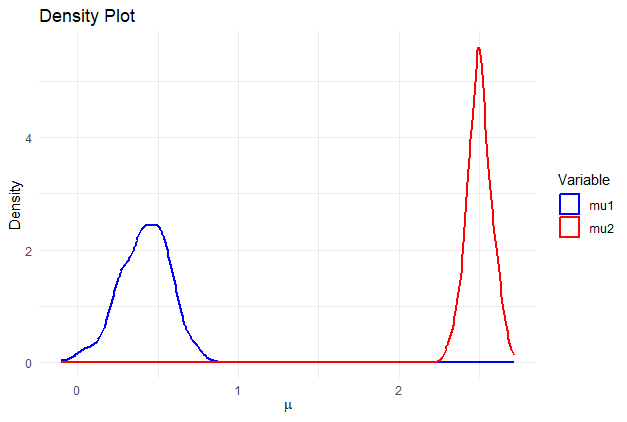
\includegraphics[width=340pt, height=200pt]{Chapters/chapter11/figures/Sim1LSI.png}
	\caption[List of figure caption goes here]{Posterior distributions: Mean parameters, population values $\beta_{01}=0.5$ and $\beta_{02}=1$.}\label{figMean1}
\end{figure}

We perform the same exercise assuming $\beta_{01}=0.5$ and $\beta_{02}=1$. Figure \ref{figMean2} shows the posterior densities, where we observe significant overlap. The posterior means are 0.77 in both cases, with 95\% credible intervals of (0.40, 1.05) and (-0.44, 1.71). The posterior mean of the probability is 0.84. 
 
\begin{figure}[!h]
	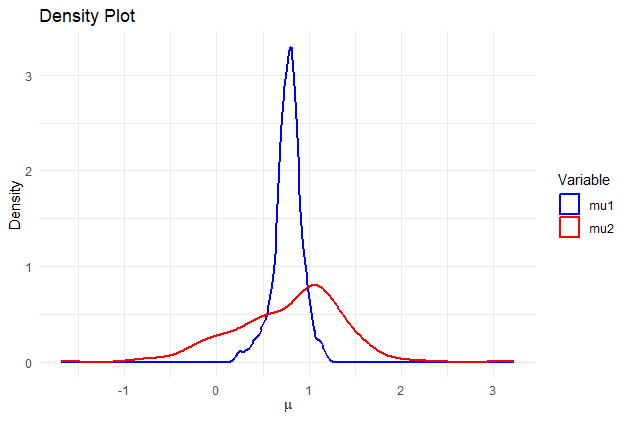
\includegraphics[width=340pt, height=200pt]{Chapters/chapter11/figures/Sim2LSI.png}
	\caption[List of figure caption goes here]{Posterior distributions: Mean parameters, population values $\beta_{01}=0.5$ and $\beta_{02}=1$.}\label{figMean2}
\end{figure}

In the second setting, the posterior draws of the Gibbs sampler can switch between the two means because they are relatively close. This situation contrasts with the first example, where there is a relatively large separation between the means. The key point is that, given a sufficiently large number of Gibbs sampler iterations, the algorithm should eventually explore the entire parameter space and encounter the label-switching issue. This occurs because the true posterior distribution is bimodal, meaning that both posterior chains should exhibit similar behavior. 

We can implement \textit{random permutation of latent classes} to address this issue. This involves sampling a random permutation of the labels at each iteration of the MCMC algorithm. For example, with three clusters, there are $3! = 6$ possible label permutations. Let the permutations be labeled as $\bm{p}_k=\left\{p_k(1),p_k(2),\dots,p_k(H)\right\}, k=1,2,\dots,H!$. At the end of each iteration in the MCMC algorithm, we randomly select one of the permutations $\bm{p}_k$ and replace the cluster probabilities $\lambda_1^{(s)},\dots,\lambda_H^{(s)}$ with $\lambda_{p_k(1)}^{(s)},\dots,\lambda_{p_k(H)}^{(s)}$. We apply the same permutation to $\bm{\beta}^{(s)}$, $\sigma^{2(s)}$, and $\bm{\psi}_{i}^{(s)}$, for $i=1,2,\dots,n$. The following algorithm illustrates how to implement this in our simple example.

\begin{tcolorbox}[enhanced,width=4.67in,center upper,
	fontupper=\large\bfseries,drop shadow southwest,sharp corners]
	\textit{R code. Simulation exercise: Random permutation of latent classes}
	\begin{VF}
		\begin{lstlisting}[language=R]
###### Permutations ######
rm(list = ls()); set.seed(010101); library(ggplot2)
# Simulate data from a 2-component mixture model
n <- 500
z <- rbinom(n, 1, 0.75)  # Latent class indicator
y <- ifelse(z == 0, rnorm(n, 0.5, 1), rnorm(n, 2.5, 1))
# Hyperparameters
mu0 <- 0; sig2mu0 <- 10; H <- 2; a0h <- rep(1/H, H)
# MCMC parameters
mcmc <- 2000; burnin <- 500
tot <- mcmc + burnin; thin <- 2
# Gibbs sampling functions
Postmu <- function(yh){
	Nh <- length(yh)
	sig2mu <- (1/sig2mu0 + Nh)^(-1)
	mun <- sig2mu*(mu0/sig2mu0 + sum(yh))
	mu <- rnorm(1, mun, sig2mu^0.5)
	return(mu)
}
PostPsi <- matrix(NA, tot, n); PostMu <- matrix(NA, tot, H)
PostLambda <- rep(NA, tot)
Id1 <- which(y <= 1); Id2 <- which(y > 1)
N1 <- length(Id1); N2 <- length(Id2)
Lambda <- c(N1/n, N2/n); MU <- c(mean(y[Id1]), mean(y[Id2]))
Psi <- rep(NA, n); per1 <- c(1,2); per2 <- c(2,1)
pb <- winProgressBar(title = "progress bar", min = 0, max = tot, width = 300)
for(s in 1:tot){
	for(i in 1:n){
		lambdai <- NULL
		for(h in 1:H){
			lambdaih <- Lambda[h]*dnorm(y[i], MU[h], 1)
			lambdai <- c(lambdai, lambdaih)
		}
		Psi[i] <- sample(1:H, 1, prob = lambdai)
	}
	for(h in 1:H){
		idh <- which(Psi == h)
		MU[h] <- Postmu(yh = y[idh])
	}
	Lambda <- MCMCpack::rdirichlet(1, a0h + table(Psi))
	# Permutations
	labels <- sample(1:2, 1, prob = c(0.5, 0.5))
	if(labels == 2){
		Lambda <- Lambda[per2]
		MU <- MU[per2]
		for(i in 1:n){
			if(Psi[i] == 1){Psi[i] <- 2
			}else{Psi[i] <- 1}
		}
	}
	PostPsi[s, ] <- Psi; PostMu[s,] <- MU
	PostLambda[s] <- Lambda[1]
	setWinProgressBar(pb, s, title=paste( round(s/tot*100, 0),"% done"))
}
close(pb)\end{lstlisting}
	\end{VF}
\end{tcolorbox}

\begin{tcolorbox}[enhanced,width=4.67in,center upper,
	fontupper=\large\bfseries,drop shadow southwest,sharp corners]
	\textit{R code. Simulation exercise: Random permutation of latent classes}
	\begin{VF}
		\begin{lstlisting}[language=R]
keep <- seq(burnin, tot, thin)
PosteriorMUs <- coda::mcmc(PostMu[keep,])
summary(PosteriorMUs)
plot(PosteriorMUs)
dfMU <- data.frame(mu1 = PostMu[keep,1], mu2 = PostMu[keep,2])
# Plot
require(latex2exp)
ggplot(dfMU) +
geom_density(aes(x = mu1, color = "mu1"), linewidth = 1) +  # First density plot
geom_density(aes(x = mu2, color = "mu2"), linewidth = 1) +  # Second density plot
labs(title = "Density Plot", x = TeX("$\\mu$"), y = "Density", color = "Variable") +
theme_minimal() +
scale_color_manual(values = c("mu1" = "blue", "mu2" = "red"))  # Custom colors
PosteriorLAMBDA <- coda::mcmc(PostLambda[keep])
summary(PosteriorLAMBDA)
plot(PosteriorLAMBDA)
		\end{lstlisting}
	\end{VF}
\end{tcolorbox}

Figure \ref{figMeanPerm} shows the posterior distributions from the random permutation of latent classes in the first simulation setting. We observe that both posterior distributions look similar.

\begin{figure}[!h]
	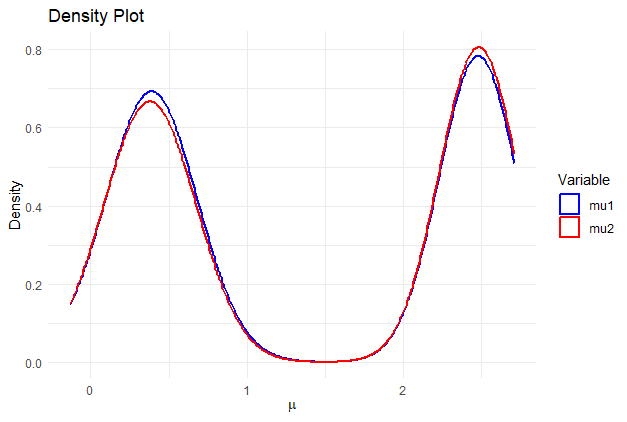
\includegraphics[width=340pt, height=200pt]{Chapters/chapter11/figures/Permutation.png}
	\caption[List of figure caption goes here]{Posterior distributions: Mean parameters, population values $\beta_{01}=0.5$ and $\beta_{02}=2.5$.}\label{figMeanPerm}
\end{figure}
 
In the following setting we simulate a simple regression mixture with two components such that $\psi_{i1}\sim \text{Ber}(0.5)$, consequently, $\psi_{i2}=1-\psi_{i1}$, and assume one regressor, $x_i\sim N(0,1)$, $i=1,2,\dots,1,000$. Then, 
$$p(y_i \mid \bm{x}_i) = 
0.5 \phi(y_i \mid 2+1.5x_i,1^2)+0.5 \phi(y_i \mid -1+0.5x_i,0.8^2).$$

The following code shows how to perform inference in this model, assuming $N(0,5)$ and $N(0,2)$ priors for the intercepts and slopes, respectively. Additionally, we use a $Cauchy(0,2)$ prior truncated at 0 for the standard deviations, and a $Dirichlet(1,1)$ prior for the probabilities. We use the \textit{brms} package in \textbf{R}, which in turn uses \textit{Stan}, setting number of MCMC iterations 2,000, a burn-in (warm-up) equal to 1,000, and 4 chains. Remember that \textit{Stan} software uses Hamiltonian Monte Carlo.

The following code performs inference in this simulation from scratch using Gibbs sampling. We do not implement the random permutation of latent classes algorithm for facilitating exposition and comparability with the results from the package \textit{brms}. We use non-informative priors, setting $\alpha_{h0}=\delta_{h0}=0.01$, $\bm{\beta}_{h0}=\bm{0}_2$, $\bm{B}_{h0}=\bm{I}_2$, and $\bm{\alpha}_0=[1/2 \ 1/2]^{\top}$. The number of MCMC iterations is 5,000, the burn-in is 1,000, and the thinning parameter is 2. In general, the Gibbs sampler appears to yield good posterior results as all 95\% intervals encompass the population parameters. 

\begin{tcolorbox}[enhanced,width=4.67in,center upper,
	fontupper=\large\bfseries,drop shadow southwest,sharp corners]
	\textit{R code. Simulation exercise: Gaussian mixture with 2 components using Hamiltonian Monte Carlo}
	\begin{VF}
		\begin{lstlisting}[language=R]
####### Simulation exercise: Gaussian mixture: 2 components #############
rm(list = ls())
set.seed(010101)
library(brms)
library(ggplot2)

# Simulate data from a 2-component mixture model
n <- 1000
x <- rnorm(n)
z <- rbinom(n, 1, 0.5)  # Latent class indicator
y <- ifelse(z == 0, rnorm(n, 2 + 1.5*x, 1), rnorm(n, -1 + 0.5*x, 0.8))
data <- data.frame(y, x)

# Plot
ggplot(data, aes(x = y)) +
geom_density(fill = "blue", alpha = 0.3) +  # Density plot with fill color
labs(title = "Density Plot", x = "y", y = "Density") +
theme_minimal()

# Define priors
priors <- c(
set_prior("normal(0, 5)", class = "Intercept", dpar = "mu1"),  # First component intercept
set_prior("normal(0, 5)", class = "Intercept", dpar = "mu2"),  # Second component intercept
set_prior("normal(0, 2)", class = "b", dpar = "mu1"),  # First component slope
set_prior("normal(0, 2)", class = "b", dpar = "mu2"),  # Second component slope
set_prior("cauchy(0, 2)", class = "sigma1", lb = 0),  # First component sigma
set_prior("cauchy(0, 2)", class = "sigma2", lb = 0),  # Second component sigma
set_prior("dirichlet(1, 1)", class = "theta")  # Mixing proportions
)

# Fit a 2-component Gaussian mixture regression model
fit <- brm(
bf(y ~ 1 + x, family = mixture(gaussian, gaussian)),  # Two normal distributions
data = data,
prior = priors,
chains = 4, iter = 2000, warmup = 1000, cores = 4
)
prior_summary(fit) # Summary of priors
summary(fit) # Summary of posterior draws
plot(fit) # Plots of posterior draws
		\end{lstlisting}
	\end{VF}
\end{tcolorbox}

\begin{tcolorbox}[enhanced,width=4.67in,center upper,
	fontupper=\large\bfseries,drop shadow southwest,sharp corners]
	\textit{R code. Simulation exercise: Gaussian mixture with 2 components using Gibbs sampling}
	\begin{VF}
		\begin{lstlisting}[language=R]
########### Perform inference from scratch ###############
rm(list = ls()); set.seed(010101)
library(brms); library(ggplot2)
# Simulate data from a 2-component mixture model
n <- 1000
x <- rnorm(n)
z <- rbinom(n, 1, 0.5)  # Latent class indicator
y <- ifelse(z == 0, rnorm(n, 2 + 1.5*x, 1), rnorm(n, -1 + 0.5*x, 0.8))
# Hyperparameters
d0 <- 0.001; a0 <- 0.001
b0 <- rep(0, 2); B0 <- diag(2); B0i <- solve(B0)
a01 <- 1/2; a02 <- 1/2
# MCMC parameters
mcmc <- 5000; burnin <- 1000
tot <- mcmc + burnin; thin <- 2
# Gibbs sampling functions
PostSig2 <- function(Betah, Xh, yh){
	Nh <- length(yh); an <- a0 + Nh
	dn <- d0 + t(yh - Xh%*%Betah)%*%(yh - Xh%*%Betah)
	sig2 <- invgamma::rinvgamma(1, shape = an/2, rate = dn/2)
	return(sig2)
}
PostBeta <- function(sig2h, Xh, yh){
	Bn <- solve(B0i + sig2h^(-1)*t(Xh)%*%Xh)
	bn <- Bn%*%(B0i%*%b0 + sig2h^(-1)*t(Xh)%*%yh)
	Beta <- MASS::mvrnorm(1, bn, Bn)
	return(Beta)
}
PostBetas1 <- matrix(0, mcmc+burnin, 2)
PostBetas2 <- matrix(0, mcmc+burnin, 2)
PostSigma21 <- rep(0, mcmc+burnin)
PostSigma22 <- rep(0, mcmc+burnin)
PostPsi <- matrix(0, mcmc+burnin, n)
PostLambda <- rep(0, mcmc+burnin)
Id1 <- which(y<1) # 1 is from inspection of the density plot of y 
N1 <- length(Id1); Lambda1 <- N1/n
Id2 <- which(y>=1)
N2 <- length(Id2); Lambda2 <- N2/n
Reg1 <- lm(y ~ x, subset = Id1)
SumReg1 <- summary(Reg1); Beta1 <- Reg1$coefficients
sig21 <- SumReg1$sigma^2 
Reg2 <- lm(y ~ x, subset = Id2); SumReg2 <- summary(Reg2)
Beta2 <- Reg2$coefficients
sig22 <- SumReg2$sigma^2
X <- cbind(1, x); Psi <- rep(NA, n)
\end{lstlisting}
	\end{VF}
\end{tcolorbox}
 
\begin{tcolorbox}[enhanced,width=4.67in,center upper,
	fontupper=\large\bfseries,drop shadow southwest,sharp corners]
	\textit{R code. Simulation exercise: Gaussian mixture with 2 components using Gibbs sampling}
	\begin{VF}
		\begin{lstlisting}[language=R]
for(s in 1:tot){
	for(i in 1:n){
		lambdai1 <- Lambda1*dnorm(y[i], X[i,]%*%Beta1, sig21^0.5)
		lambdai2 <- Lambda2*dnorm(y[i], X[i,]%*%Beta2, sig22^0.5)
		Psi[i] <- sample(c(1,2), 1, prob = c(lambdai1, lambdai2))
	}
	PostPsi[s, ] <- Psi
	Id1 <- which(Psi == 1); Id2 <- which(Psi == 2)
	N1 <- length(Id1); N2 <- length(Id2)
	sig21 <- PostSig2(Betah = Beta1, Xh = X[Id1, ], yh = y[Id1])
	sig22 <- PostSig2(Betah = Beta2, Xh = X[Id2, ], yh = y[Id2])
	PostSigma21[s] <- sig21; PostSigma22[s] <- sig22
	Beta1 <- PostBeta(sig2h = sig21, Xh = X[Id1, ], yh = y[Id1])
	Beta2 <- PostBeta(sig2h = sig22, Xh = X[Id2, ], yh = y[Id2])
	PostBetas1[s,] <- Beta1; PostBetas2[s,] <- Beta2
	Lambda <- MCMCpack::rdirichlet(1, c(a01 + N1, a02 + N2))
	Lambda1 <- Lambda[1]; Lambda2 <- Lambda[2]
	PostLambda[s] <- Lambda1 
}
keep <- seq((burnin+1), tot, thin)
PosteriorBetas1 <- coda::mcmc(PostBetas1[keep,])
summary(PosteriorBetas1)
plot(PosteriorBetas1)
PosteriorBetas2 <- coda::mcmc(PostBetas2[keep,])
summary(PosteriorBetas2)
plot(PosteriorBetas2)
PosteriorSigma21 <- coda::mcmc(PostSigma21[keep])
summary(PosteriorSigma21)
plot(PosteriorSigma21)
PosteriorSigma22 <- coda::mcmc(PostSigma22[keep])
summary(PosteriorSigma22)
plot(PosteriorSigma22)
\end{lstlisting}
	\end{VF}
\end{tcolorbox}

Let's perform another simulation exercise in which we conduct a semi-parametric analysis where the stochastic error follows a Student's t-distribution with 3 degrees of freedom. Specifically,  
\begin{align*}
	y_i &= 1 - 0.5x_{i1} + 1.5x_{i2} + \mu_i, \ i=1,2,\dots,500.
\end{align*}
The variables $x_{i1}$ and $x_{i2}$ are standard normally distributed. Let's set $H=5$, and use non-informative priors setting $\alpha_{h0}=\delta_{h0}=0.01$, $\bm{\beta}_0=\bm{0}_2$, $\bm{B}_0=\bm{I}_2$, $\mu_{h0}=0$, $\sigma^2_{\mu 0}=10$ and $\bm{\alpha}_0=[1/H \ \dots \ 1/H]^{\top}$. Use 6,000 MCMC iterations, burn-in equal to 4,000, and thinning parameter equal to 2. In this exercise, there is no need to address the label-switching issue, as we are not specifically interested in the individual components of the posterior distributions of the clusters. 

We can see from the posterior estimates that three components disappear after the burn-in iterations. The 95\% credible intervals encompass the population values of the slope parameters. The 95\% credible intervals for the probabilities are (0.70, 0.89) and (0.11, 0.30), and the 95\% credible interval for the weighted average of the intercepts encompasses the population parameter.

\begin{tcolorbox}[enhanced,width=4.67in,center upper,
	fontupper=\large\bfseries,drop shadow southwest,sharp corners]
	\textit{R code. Simulation exercise: Semi-parametric model using Gibbs sampling}
	\begin{VF}
		\begin{lstlisting}[language=R]
rm(list = ls()); set.seed(010101)
library(ggplot2)
# Simulate data from a 2-component mixture model
n <- 500
x1 <- rnorm(n); x2 <- rnorm(n)
X <- cbind(x1,x2); B <- c(-0.5, 1.5)
u <- rt(n, 3); y <- 1 + X%*%B + u
Reg <- lm(y ~ X)
Res <- Reg$residuals
data <- data.frame(Res)
# Plot
ggplot(data, aes(x = Res)) +
geom_density(fill = "blue", alpha = 0.3) +  # Density plot with fill color
labs(title = "Density Plot", x = "Residuals", y = "Density") +
theme_minimal()
# Hyperparameters
d0 <- 0.001; a0 <- 0.001; b0 <- rep(0, 2)
B0 <- diag(2); B0i <- solve(B0)
mu0 <- 0; sig2mu0 <- 10; H <- 5; a0h <- rep(1/H, H)
# MCMC parameters
mcmc <- 2000; burnin <- 4000
tot <- mcmc + burnin; thin <- 2
# Gibbs sampling functions
PostSig2 <- function(Beta, muh, Xh, yh){
	Nh <- length(yh); an <- a0 + Nh
	dn <- d0 + t(yh - muh - Xh%*%Beta)%*%(yh - muh - Xh%*%Beta)
	sig2 <- invgamma::rinvgamma(1, shape = an/2, rate = dn/2)
	return(sig2)
}
PostBeta <- function(sig2, mu, X, y, Psi){
	XtX <- matrix(0, 2, 2); Xty <- matrix(0, 2, 1)
	Hs <- length(mu)
	for(h in 1:Hs){
		idh <- which(Psi == h)
		if(length(idh) == 1){
			Xh <- matrix(X[idh,], 1, 2)
			XtXh <- sig2[h]^(-1)*t(Xh)%*%Xh
			yh <- y[idh]
			Xtyh <- sig2[h]^(-1)*t(Xh)%*%(yh - mu[h])
		}else{
			Xh <- X[idh,]
			XtXh <- sig2[h]^(-1)*t(Xh)%*%Xh
			yh <- y[idh]
			Xtyh <- sig2[h]^(-1)*t(Xh)%*%(yh - mu[h])
		}
		XtX <- XtX + XtXh; Xty <- Xty + Xtyh
	}
	Bn <- solve(B0i + XtX); bn <- Bn%*%(B0i%*%b0 + Xty)
	Beta <- MASS::mvrnorm(1, bn, Bn)
	return(Beta)
}
\end{lstlisting}
	\end{VF}
\end{tcolorbox}

\begin{tcolorbox}[enhanced,width=4.67in,center upper,
	fontupper=\large\bfseries,drop shadow southwest,sharp corners]
	\textit{R code. Simulation exercise: Semi-parametric model using Gibbs sampling}
	\begin{VF}
		\begin{lstlisting}[language=R]
Postmu <- function(sig2h, Beta, Xh, yh){
	Nh <- length(yh)
	sig2mu <- (1/sig2mu0 + Nh/sig2h)^(-1)
	mun <- sig2mu*(mu0/sig2mu0 + sum((yh - Xh%*%Beta))/sig2h)
	mu <- rnorm(1, mun, sig2mu^0.5)
	return(mu)
}
PostBetas <- matrix(0, mcmc+burnin, 2)
PostPsi <- matrix(0, mcmc+burnin, n)
PostSigma2 <- list(); PostMu <- list()
PostLambda <- list()
Resq <- quantile(Res, c(0.2, 0.4, 0.6, 0.8))
Id1 <- which(Res <= Resq[1])
Id2 <- which(Res > Resq[1] & Res <= Resq[2])
Id3 <- which(Res > Resq[2] & Res <= Resq[3])
Id4 <- which(Res > Resq[3] & Res <= Resq[4])
Id5 <- which(Res > Resq[4])
Nh <- rep(n/H, H); Lambda <- rep(1/H, H)
MU <- c(mean(Res[Id1]), mean(Res[Id2]), mean(Res[Id3]), mean(Res[Id4]), mean(Res[Id5]))
Sig2 <- c(var(Res[Id1]), var(Res[Id2]), var(Res[Id3]), var(Res[Id4]), var(Res[Id5]))
Beta <- Reg$coefficients[2:3]
Psi <- rep(NA, n); Hs <- length(MU)
pb <- winProgressBar(title = "progress bar", min = 0, max = tot, width = 300)
for(s in 1:tot){
	for(i in 1:n){
		lambdai <- NULL
		for(h in 1:Hs){
			lambdaih <- Lambda[h]*dnorm(y[i] - X[i,]%*%Beta, MU[h], Sig2[h]^0.5)
			lambdai <- c(lambdai, lambdaih)
		}
		Psi[i] <- sample(1:Hs, 1, prob = lambdai)
	}
	PostPsi[s, ] <- Psi
	Hs <- length(table(Psi))
	for(h in 1:Hs){
		idh <- which(Psi == h)
		Sig2[h] <- PostSig2(Beta = Beta, muh = MU[h], Xh = X[idh,], yh = y[idh])
		MU[h] <- Postmu(sig2h = Sig2[h], Beta = Beta, Xh = X[idh,], yh = y[idh])
	}
	PostSigma2[[s]] <- Sig2
	PostMu[[s]] <- MU 
	Beta <- PostBeta(sig2 = Sig2, mu = MU, X = X, y = y, Psi = Psi)
	PostBetas[s,] <- Beta
	Lambda <- sort(MCMCpack::rdirichlet(1, a0h[1:Hs] + table(Psi)), decreasing = TRUE)
	PostLambda[[s]] <- Lambda
	setWinProgressBar(pb, s, title=paste( round(s/tot*100, 0),"% done"))
}
close(pb)
\end{lstlisting}
	\end{VF}
\end{tcolorbox}

\begin{tcolorbox}[enhanced,width=4.67in,center upper,
	fontupper=\large\bfseries,drop shadow southwest,sharp corners]
	\textit{R code. Simulation exercise: Semi-parametric model using Gibbs sampling}
	\begin{VF}
		\begin{lstlisting}[language=R]
keep <- seq(burnin, tot, thin)
PosteriorBetas <- coda::mcmc(PostBetas[keep,])
summary(PosteriorBetas)
plot(PosteriorBetas)
PosteriorPsi <- PostPsi[keep,]
Clusters <- sapply(1:length(keep), function(i){length(table(PosteriorPsi[i,]))})
NClus <- 2
PosteriorSIGMA <- matrix(NA, length(keep), NClus)
PosteriorMU <- matrix(NA, length(keep), NClus)
PosteriorLAMBDA <- matrix(NA, length(keep), NClus)
l <- 1
for (s in keep){
	PosteriorSIGMA[l,] <- PostSigma2[[s]][1:NClus]
	PosteriorMU[l,] <- PostMu[[s]][1:NClus]
	PosteriorLAMBDA[l,] <- PostLambda[[s]][1:NClus]
	l <- l + 1
}

summary(coda::mcmc(PosteriorSIGMA))
summary(coda::mcmc(PosteriorMU))
summary(coda::mcmc(PosteriorLAMBDA))
\end{lstlisting}
	\end{VF}
\end{tcolorbox}


\subsection{Direchlet processes}\label{sec11_12}

\section{Non-parametric generalized additive models}\label{sec11_2}
%\section{Additive non-parametric structure}\label{sec11_1}
%\subsection{Partial linear model}\label{sec11_21}

\section{Summary}\label{sec11_3}

\section{Exercises}\label{sec11_4}

\begin{enumerate}
	\item Simulate a semi-parametric regression where  
	\begin{align*}
		y_i &= 0.5x_{i1} - 1.2x_{i2} + \mu_i, \\
		p(\mu_i) &= 
		0.3 \phi(\mu_i \mid -0.5,0.5^2) + 0.7 \phi(\mu_i \mid 1,0.8^2).		
	\end{align*}
	Assume that $x_{i1}$ and $x_{i2}$ follow a standard normal distribution and that the sample size is 1,000. Perform inference in this model assuming that the number of components is unknown. Start with $H=5$ and use non-informative priors, setting $\alpha_{h0}=\delta_{h0}=0.01$, $\bm{\beta}_0=\bm{0}_2$, $\bm{B}_0=\bm{I}_2$, $\mu_{h0}=0$, $\sigma^2_{\mu 0}=10$, and $\bm{\alpha}_0=[1/H \ \dots \ 1/H]^{\top}$. Use 6,000 MCMC iterations, a burn-in period of 4,000, and a thinning parameter of 2. Compare the population parameters with the posterior estimates and plot the population density along with the posterior density estimate of $\bm{\mu}$ (the mean, and the 95\% credible interval).
	
	\item 
	

  
\end{enumerate}

